% =====================================================================
%  Neural Networks -- Manara University
%  Text-to-Image Generation on CUB-200-2011
%  Baraa Lazkani, Humam Yehia
% =====================================================================
\documentclass[11pt,a4paper]{article}

\usepackage[utf8]{inputenc}
\usepackage[T1]{fontenc}
\usepackage{lmodern}   % scalable Type1 fonts (microtype expansion needs these)
\usepackage[margin=2.4cm]{geometry}
\usepackage{graphicx}
\usepackage{float}
\usepackage{xcolor}
\usepackage[table]{xcolor}
\usepackage{colortbl}
\usepackage{booktabs}
\usepackage{tabularx}
\usepackage{amsmath,amssymb}
\usepackage{enumitem}
\usepackage{titlesec}
\usepackage{fancyhdr}
\usepackage{caption}
\usepackage{subcaption}
\usepackage[most]{tcolorbox}
\usepackage{tikz}
\usepackage{pgfplots}
\usepackage{listings}
\usepackage{microtype}
\usepackage[hidelinks]{hyperref}

\pgfplotsset{compat=1.18}
\usetikzlibrary{arrows.meta, positioning, fit, backgrounds, calc}

% --- global list compaction (long-form best practice) ---
\setlist[itemize]{nosep, leftmargin=*, topsep=2pt, partopsep=0pt}
\setlist[enumerate]{nosep, leftmargin=*, topsep=2pt, partopsep=0pt}

% --- colours ---
\definecolor{accent}{HTML}{C2410C}
\definecolor{ink}{HTML}{1F2937}
\definecolor{soft}{HTML}{F3F4F6}
\definecolor{line}{HTML}{D1D5DB}
\definecolor{good}{HTML}{15803D}
\definecolor{bad}{HTML}{B91C1C}

\titleformat{\section}{\Large\bfseries\color{accent}}{\thesection}{0.7em}{}
\titleformat{\subsection}{\large\bfseries\color{ink}}{\thesubsection}{0.6em}{}

\pagestyle{fancy}
\fancyhf{}
\fancyhead[L]{\small\textcolor{ink}{Text-to-Image Generation on CUB-200-2011}}
\fancyhead[R]{\small\textcolor{ink}{Neural Networks --- Manara University}}
\fancyfoot[C]{\small\thepage}
\renewcommand{\headrulewidth}{0.4pt}

\captionsetup{font=small, labelfont={bf,color=accent}}

\lstset{
  basicstyle=\ttfamily\scriptsize,
  backgroundcolor=\color{soft},
  frame=single, rulecolor=\color{line},
  breaklines=true, columns=fullflexible,
  showstringspaces=false, xleftmargin=6pt, framexleftmargin=6pt
}

% key-finding box
\newtcolorbox{finding}[1]{colback=accent!5, colframe=accent!70, title={\textbf{#1}},
  fonttitle=\bfseries, boxrule=0.8pt, left=6pt, right=6pt, top=4pt, bottom=4pt}
\newtcolorbox{lesson}[1]{colback=good!5, colframe=good!60, title={\textbf{#1}},
  fonttitle=\bfseries, boxrule=0.8pt, left=6pt, right=6pt, top=4pt, bottom=4pt}

\newcommand{\step}[1]{\section{#1}}

\begin{document}

% =====================  TITLE  =====================
\begin{titlepage}
\centering
\vspace*{1.6cm}

{\Large\scshape Manara University}\\[0.3cm]
{\large Faculty of Engineering}\\[1.6cm]

\textcolor{accent}{\rule{\textwidth}{2pt}}\\[0.7cm]
{\Huge\bfseries Text-to-Image Generation}\\[0.45cm]
{\LARGE on the CUB-200-2011 Dataset}\\[0.8cm]
{\large\itshape Training a Diffusion Transformer from Scratch and\\
Fine-Tuning Stable Diffusion 1.5 with LoRA\\
on a Single 8\,GB Laptop GPU}\\[0.6cm]
\textcolor{accent}{\rule{\textwidth}{2pt}}\\[1.8cm]

{\large\bfseries Course:} {\large Neural Networks}\\[1.6cm]

{\large\bfseries Submitted by}\\[0.5cm]
{\Large Baraa Lazkani}\\[0.35cm]
{\Large Humam Yehia}\\[2.4cm]

{\large \today}

\vfill
\end{titlepage}

% =====================  ABSTRACT  =====================
\section*{Abstract}
\addcontentsline{toc}{section}{Abstract}

This report documents the design, implementation, training and evaluation of a
complete text-to-image generation system built on the CUB-200-2011 bird dataset.
Two models were produced. The first is a \textbf{diffusion transformer of 55.6
million parameters trained entirely from scratch}, with no pretrained denoiser
weights, using a rectified flow-matching objective. The second is
\textbf{Stable Diffusion 1.5 fine-tuned with LoRA adapters}, updating only 3.19
million parameters, or $0.37\%$ of the network.

The organising idea of the project is that both models share one latent space
and one text-conditioning space. The image autoencoder and the CLIP text encoder
are frozen and common to both, so only the denoiser differs. This makes the
comparison between them genuinely controlled: when the same caption and the same
starting noise are pushed through both, every difference in the output is
attributable to the denoiser rather than to the surrounding pipeline.

All work was carried out on a single laptop GPU with 8\,GB of video memory. This
constraint shaped nearly every design decision, and the report treats it as a
first-class part of the engineering problem rather than a footnote.

The headline result is a genuine trade-off rather than a clean win. The
fine-tuned model produces sharper, more photorealistic images and achieves the
better CLIP score of $0.3099$. The from-scratch model scores lower at $0.2920$
and works at half the resolution, yet it follows the caption more faithfully,
correctly altering the intended attribute in four of four controlled tests where
the fine-tuned model managed roughly two. We argue that this is not a defect in
either model but a direct consequence of what each one knows.

\vspace{0.4cm}
\noindent\textbf{Keywords:} diffusion models, diffusion transformers, rectified
flow, classifier-free guidance, LoRA, latent diffusion, text-to-image synthesis,
CUB-200-2011.

\newpage
\tableofcontents
\newpage

% =====================  INTRO  =====================
\section{Introduction and Objectives}

Text-to-image generation has become one of the most visible applications of deep
learning, but the models that dominate public attention are trained on hundreds
of millions of images using clusters of high-end accelerators. That scale hides
the mechanics. A student who only ever calls a pretrained pipeline learns the
API, not the model.

The objective of this project was therefore deliberately split in two. We wanted
to \emph{build} a text-conditional diffusion model from first principles ---
architecture, noise schedule, training objective, sampler and guidance
mechanism, all written by hand --- and we wanted to \emph{measure} it against the
pragmatic industry approach of adapting a large pretrained model. Doing only the
first risks producing something that looks impressive but cannot be judged.
Doing only the second risks learning nothing about how diffusion actually works.

\begin{finding}{The central research question}
Given a fixed, modest compute budget and a narrow domain, how does a small
diffusion transformer trained from random initialisation compare against a large
pretrained model adapted to the same domain --- not only in image quality, but
in \emph{faithfulness to the text prompt}?
\end{finding}

The dataset chosen was CUB-200-2011, which pairs 11{,}788 photographs of 200
bird species with ten human-written captions each. Its captions are unusually
attribute-dense, describing colour, body part and bill shape explicitly. This
makes it possible to test text conditioning in a controlled way that open-domain
datasets do not permit: two captions can be constructed that differ in exactly
one word, and the model's response to that single word can be observed directly.

The remainder of this report is organised as a sequence of steps, in the order
the work was actually carried out. Each step states what was done, why it was
done that way, and what was measured. Section~\ref{sec:problems} is devoted
entirely to the engineering faults encountered, because several of them were
silent --- they produced no error message and no obviously wrong output --- and
finding them was a substantial part of the work.

% =====================  STEP 1  =====================
\step{Step 1: Establishing the Hardware Budget}

Every subsequent decision in this project follows from the hardware, so the
hardware was measured before anything was designed.

\begin{table}[htbp]
\centering
\caption{Measured hardware and software environment.}
\begin{tabularx}{0.92\textwidth}{@{}lX@{}}
\toprule
\textbf{Component} & \textbf{Specification} \\
\midrule
GPU & NVIDIA GeForce RTX 5050 Laptop, \textbf{8\,GB VRAM}, Blackwell architecture (compute capability $12.0$, \texttt{sm\_120}) \\
System RAM & 15\,GB \\
Free disk & approximately 12\,GB at project start \\
PyTorch & \texttt{2.11.0.dev+cu130} (nightly build) \\
Precision & \texttt{bfloat16} throughout \\
\bottomrule
\end{tabularx}
\end{table}

Two properties of this environment deserve comment. First, the Blackwell
architecture is recent enough that only a PyTorch nightly build supported it at
the time of the work; a stable release would have compiled without
\texttt{sm\_120} kernels and failed at runtime. Every package installation
throughout the project therefore had to be checked to confirm it would not
silently replace that nightly.

Second, and more importantly, \textbf{8\,GB of video memory is the binding
constraint of the entire project}. Stable Diffusion XL requires roughly 7\,GB
merely to hold its weights, leaving nothing for training. Stable Diffusion 1.5
in half precision requires about 2\,GB. That single fact determined the choice
of base model, and through it the latent space, the text encoder, and the
resolution at which the from-scratch model would operate.

\begin{lesson}{Why measure rather than assume}
We used \texttt{bfloat16} rather than the more common \texttt{float16}. On
Blackwell it runs at full speed, and because it carries the same exponent range
as \texttt{float32}, it removes gradient-scaling overflow as a failure mode
entirely. Using one precision across the whole project also eliminated a class
of dtype-mismatch bugs, though as Section~\ref{sec:problems} records, not all of
them.
\end{lesson}

% =====================  STEP 2  =====================
\step{Step 2: System Architecture}
\label{sec:arch-ref}
\noindent\textit{One latent space, two denoisers.}\medskip

A text-to-image latent diffusion system has three learned components: an
autoencoder that compresses images into a latent space, a text encoder that
converts captions into conditioning vectors, and a denoiser that learns to
reverse a noising process in that latent space.

Only the third of these is interesting for this project. The autoencoder and the
text encoder are generic --- they are not specific to birds, and training them
would consume the entire compute budget without teaching anything about
diffusion. We therefore froze both and \textbf{shared them between the two
models}, leaving the denoiser as the only component that differs.

\begin{figure}[htbp]
\centering
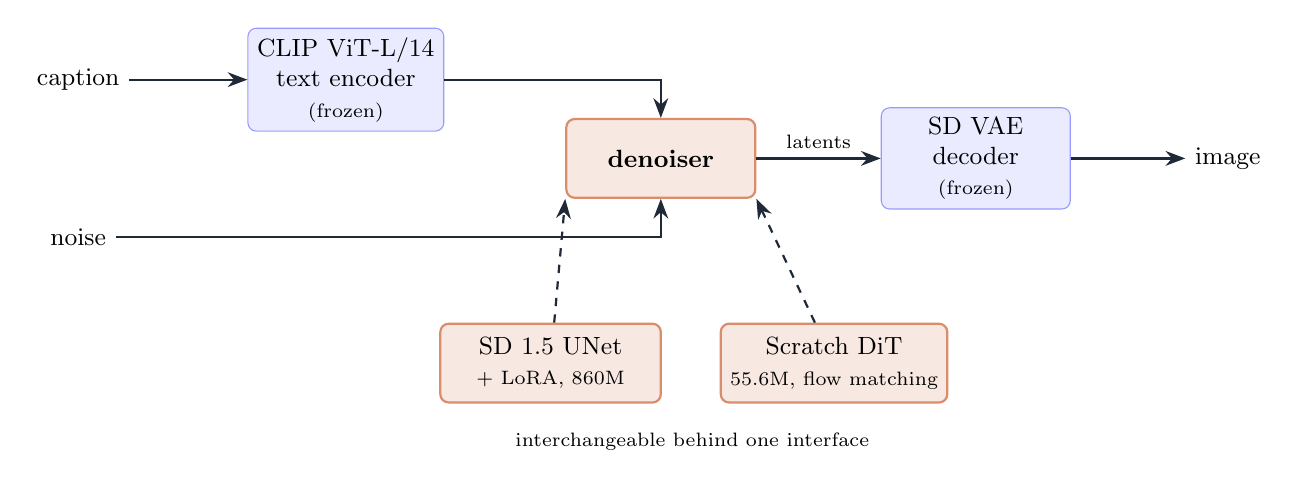
\begin{tikzpicture}[
  font=\small,
  box/.style={draw=line, fill=soft, rounded corners=3pt, minimum height=1cm, minimum width=2.4cm, align=center},
  frozen/.style={box, fill=blue!8, draw=blue!40},
  learn/.style={box, fill=accent!12, draw=accent!60, thick},
  ar/.style={-{Stealth[length=2.5mm]}, thick, draw=ink}
]
\node[frozen] (txt) at (0,1.2) {CLIP ViT-L/14\\text encoder\\{\scriptsize(frozen)}};
\node        (cap) at (-3.4,1.2) {caption};
\node        (noi) at (-3.4,-0.8) {noise};
\node[learn] (den) at (4.0,0.2) {\textbf{denoiser}};
\node[frozen] (vae) at (8.0,0.2) {SD VAE\\decoder\\{\scriptsize(frozen)}};
\node        (img) at (11.2,0.2) {image};

\draw[ar] (cap) -- (txt);
\draw[ar] (txt) -| (den.north);
\draw[ar] (noi) -| (den.south);
\draw[ar] (den) -- node[above,font=\scriptsize]{latents} (vae);
\draw[ar] (vae) -- (img);

\node[learn, minimum width=2.8cm] (a) at (2.6,-2.4) {SD 1.5 UNet\\{\scriptsize+ LoRA, 860M}};
\node[learn, minimum width=2.8cm] (b) at (6.2,-2.4) {Scratch DiT\\{\scriptsize55.6M, flow matching}};
\draw[ar, dashed] (a) -- (den.south west);
\draw[ar, dashed] (b) -- (den.south east);
\node[font=\scriptsize, align=center] at (4.4,-3.4) {interchangeable behind one interface};
\end{tikzpicture}
\caption{System architecture. The text encoder and the autoencoder are frozen
and shared; the denoiser is the only component that varies between the two
models. Because the noise, the conditioning and the decoder are identical, any
difference in output is attributable to the denoiser alone.}
\label{fig:arch}
\end{figure}

This choice pays for itself three times over. It halves the disk footprint,
since only one autoencoder and one text encoder are stored. It allows the
expensive image-encoding step to be computed once and reused by both training
runs. And it makes the final comparison methodologically sound, which is the
part that matters for a report.

In software terms the seam is a single abstract class. Both denoisers implement
the same method signature, declare what quantity they predict, and are consumed
by a sampler that dispatches on that declaration. The sampling code, the
evaluation harness and the graphical application were all written against this
interface and never branch on which model they hold.

% =====================  STEP 3  =====================
\step{Step 3: The Dataset}

CUB-200-2011 contains 11{,}788 photographs spanning 200 North American bird
species. The captions come from a separate collection by Reed et al., in which
annotators wrote ten single-sentence descriptions per image, focusing on
morphology --- plumage colour, body part, bill shape. The combination yields
\textbf{117{,}880 distinct image-text pairs} from fewer than twelve thousand
photographs.

That multiplicity matters more than it might appear. Transformers are less
sample-efficient than convolutional networks, and 11{,}788 images is a small
dataset by any generative standard. Because a different caption can be drawn for
the same image on every epoch, the effective number of training pairs is an
order of magnitude larger than the number of photographs.

\subsection{Bounding-box cropping}

CUB photographs are field photographs: the bird frequently occupies a small
fraction of a cluttered frame. A small generative model trained on raw frames
would spend much of its limited capacity modelling branches, foliage and sky.

Following the convention established by the StackGAN and AttnGAN literature, we
used the bounding-box annotations shipped with the dataset to take a square crop
centred on the bird, sized so that the bird fills approximately $75\%$ of the
frame. Where the window ran past an image edge it was shifted rather than shrunk,
so that crops remain square and retain full context.

\subsection{Data splitting}

The dataset was divided by image rather than by species, holding out $5\%$ for
validation: \textbf{11{,}199 training images and 589 validation images}. The
alternative --- holding out 50 entire species, as the Reed protocol does ---
tests generalisation to unseen birds more strictly, but costs a quarter of the
training data. At this scale, with a model learning basic image structure from
scratch, maximising training data was judged the better trade. The stricter
split remains available as a configuration option.

% =====================  STEP 4  =====================
\step{Step 4: Building the Shared Latent Space}

Diffusion in pixel space at $256\times256$ resolution would require modelling
196{,}608 dimensions per image. Latent diffusion instead compresses the image
first. The Stable Diffusion 1.5 autoencoder reduces an image by a factor of
eight in each spatial dimension into four channels, so a $256\times256$ image
becomes a $4\times32\times32$ latent --- a reduction of $48\times$.

\subsection{The asymmetry that shaped the pipeline}

A key decision concerns \emph{what to precompute}. There are two frozen
components, and they have opposite cost profiles.

\textbf{Image latents} are expensive to compute --- a full convolutional
encoder pass per image --- but cheap to store. The complete 256-pixel cache
occupies 193\,MB, and the 512-pixel cache 773\,MB.

\textbf{Text embeddings} are the reverse. A CLIP text encoder pass takes roughly
two milliseconds, but storing $117{,}880$ captions at $77\times768$ in half
precision would require approximately \textbf{14\,GB} --- more free disk than the
machine had.

The pipeline therefore precomputes latents and encodes text on the fly. This is
the single most important optimisation in the project: because the autoencoder
never enters video memory during training, the entire 8\,GB is available to the
denoiser. Without it, training a from-scratch transformer on this hardware would
not have been feasible.

Horizontal flipping is the one augmentation that survives precomputation --- a
latent cannot simply be flipped to obtain the latent of the flipped image --- so
both orientations were encoded and stored, doubling the cache but preserving the
augmentation.

% =====================  STEP 5  =====================
\step{Step 5: Verifying the Data Pipeline}
\label{sec:verify}

Before any model was trained, the latent cache was verified. This was
deliberate. Every model in this project learns to produce latents, and is judged
only after those latents pass through the decoder. If the cache is wrong ---
through a mis-applied scaling factor, a mismatched crop, or a transposed index
--- training still produces a smoothly falling loss curve while generating
nothing but noise, and the cause is extremely difficult to diagnose from that
side.

Two properties were checked. Reconstruction fidelity confirms that a cached
latent decodes back to its source image. Flip-index alignment confirms that the
second stored orientation really is the mirror of the first.

\begin{table}[htbp]
\centering
\caption{Latent cache verification. Both resolutions pass comfortably; the
threshold for acceptance was 20\,dB.}
\begin{tabular}{@{}lccc@{}}
\toprule
\textbf{Cache} & \textbf{Reconstruction PSNR} & \textbf{Flip alignment PSNR} & \textbf{Size} \\
\midrule
256\,px (DiT)  & $27.15$\,dB & $27.13$\,dB & 193\,MB \\
512\,px (LoRA) & $\mathbf{30.77}$\,dB & $30.80$\,dB & 773\,MB \\
\bottomrule
\end{tabular}
\end{table}

That the flip-alignment figure matches the reconstruction figure almost exactly
is the meaningful part: had the two stored orientations been swapped or
mis-indexed, that number would have collapsed while reconstruction stayed high.

\begin{figure}[htbp]
\centering
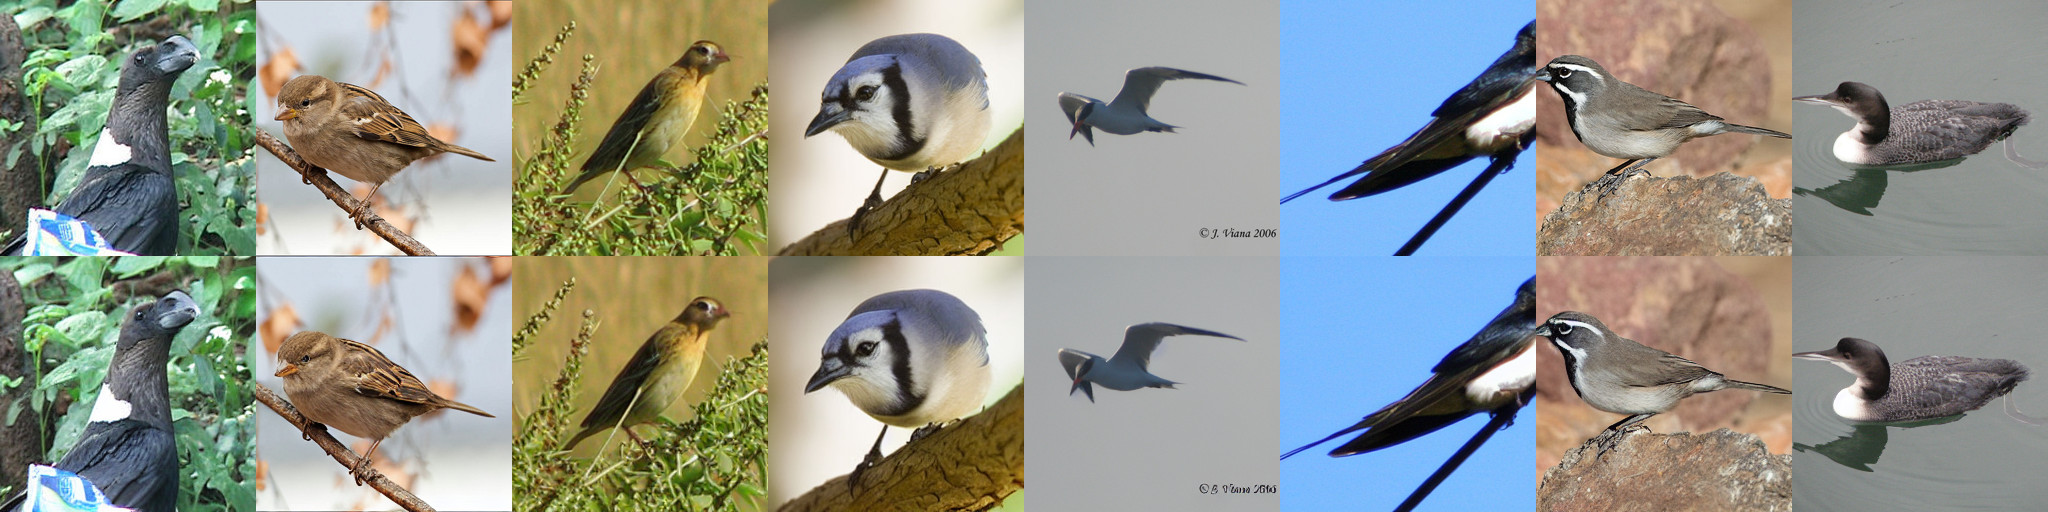
\includegraphics[width=0.95\textwidth]{figures/reconstruction_256.jpg}
\caption{Latent cache verification at 256 pixels. Top row: original
bounding-box crops. Bottom row: the same images decoded from their cached
latents. The birds are well centred by the bounding-box crop, and the only
visible degradation is in fine text (the photographers' watermarks), which is
expected of a lossy autoencoder.}
\label{fig:recon}
\end{figure}


\end{document}
